\chapter{WebSocket Application Deployment}
\label{chapter:webSocketApplicationDeployment}

\section{WebSocket Connection Types}

When deploying a WebSocket application there are special requirements that need to be taken into account. These requirements depend on the nature of the deployed applications and the traffic handled by their run-time environments. In addition, devices like reverse proxy servers, firewalls and load-balancing routers must be taken into account when designing and implementing systems that utilize the WebSocket protocol. A large proportion of the internet infrastructure is predominantly configured for HTTP traffic and not familiar with WebSocket which can introduce various challenges when deploying applications that utilize the protocol.

\subsection{Unencrypted WebSocket Traffic}

The deciding factor whether a client and a server successfully manage to establish an unencrypted WebSocket connection (\texttt{ws://} on port 80) in a production environments is usually interaction with proxy servers located on the communication path. Connections through explicit proxy servers, that a client is explicitly configured to use, will most likely lead to a successful connection upgrade during the WebSocket handshake as they are configured to allow the \texttt{CONNECT} method. WebSocket traffic that flows through transparent proxies, which intercept normal communication at the network layer without requiring any special client configuration, is likely to be dropped as the proxy is likely to remove certain header information which can lead to a failed WebSocket handshake. Even though a transparent proxy server is not configured to remove the connection header the WebSocket connection is still unlikely to succeed as it behaves differently than HTTP traffic which is what the server has mainly been configured for. This scenario will most likely be the case until the infrastructure of the Internet has more frequently be configured to handle the traffic of long-lived connections of protocols like WebSocket and HTTP/2. Figure~\ref{fig:webSocketProxyServer} shows interaction between WebSocket and different types of proxy servers and whether a successful connection establishment is likely to be successful for both encrypted and unencrypted WebSocket traffic.
\\
\begin{figure}[h!]
	\centering
	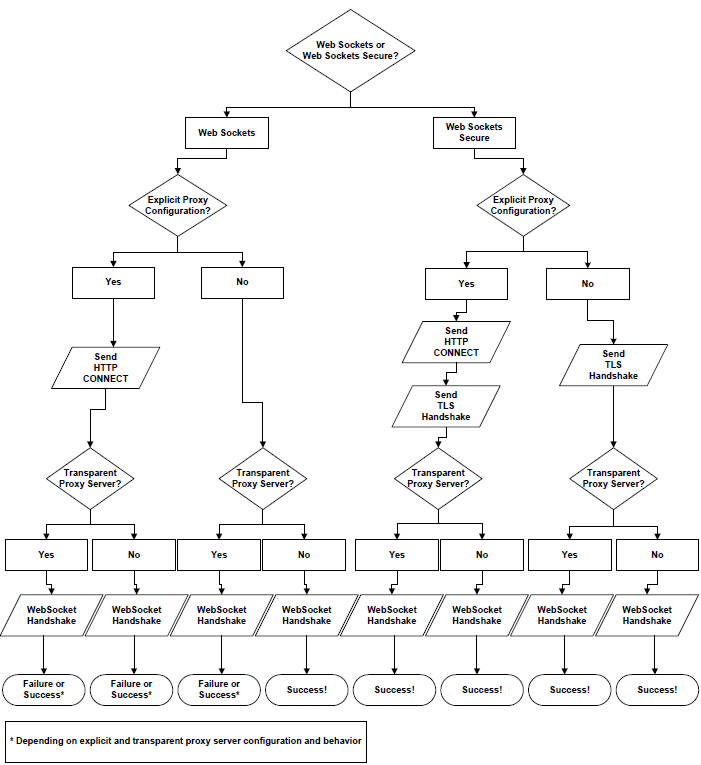
\includegraphics[width=0.8\textwidth]{images/websocketProxyServer}
	\caption{Interaction between WebSocket applications and proxy servers \cite{wang2013definitive}}
	\label{fig:webSocketProxyServer}
\end{figure}

\newpage
\subsection{Encrypted WebSocket traffic}

Encrypted WebSocket traffic (\texttt{wss://} on port 443) is more predictable than unencrypted traffic as it is less dependent on the intermediaries on the connection path. In the case of explicit proxies a TLS handshake takes place after a successful WebSocket connection upgrade handshake. Afterwards an encrypted and unhampered WebSocket communication channel is established between a client and a server. When a WebSocket connection is established in the presence of transparent proxies a successful handshake is considerably more likely as the communication is encrypted and proxies are generally configured to accept that kind of traffic. TLS encrypted traffic leads to slightly increased CPU consumption on both sides of the communication but its benefits significantly outweigh that drawback.

\subsection{Fallback Strategies and WebSocket Abstractions}

In addition to the possible issues proxy servers and other intermediaries can cause for WebSocket traffic some older browsers lack support for the protocol. Currently, all modern browsers\footnote{\url{http://caniuse.com/websocket}} support the protocol but WebSocket applications that are intended for widespread use and corporate environments, where older browsers might be common, should have a decent fallback strategy to ensure a positive user experience. Because of the uncertainty in the environment where WebSocket applications can be deployed polyfills, which are libraries that implement a standard API using legacy browser features, can be a good solution. In the case of WebSocket a polyfill library would most likely use HTTP-based communication patterns like polling or long-polling as a fallback option. Another option would be to use a plugin, like Adobe Flash, capable of establishing a full-duplex communication channel with TCP sockets. That option use usually the less favorable as it requires the user to explicitly install the plugin.
\\ \\
Engine.io\footnote{\url{https://github.com/Automattic/engine.io}} is a Node.js WebSocket implementation that adds increased reliability when establishing a WebSocket connection between a client and a server. The most important design implementation of Engine.io is that communication is initiated with a long-polling connection that is gradually upgraded to better transports that are tested during the first moments of the connection establishment. This approach to WebSocket connection establishment is based on empirical experience working with the protocol in production environments in the vicinity of proxies and other network intermediaries. Experiments even seem to indicate that a WebSocket abstraction like Engine.io can increase data throughput without a significant impact on permanence \cite{ozger2014websocket}. There are numerous other WebSocket implementations and frameworks that add different levels of abstractions and connection management. At the current moment these extensions seem to be necessary to increase the reliability of unencrypted WebSocket traffic while the majority of the underlying infrastructure of the web is still predominantly configure for HTTP-based traffic.

\subsection{WebSocket Connection Analysis}

For the analysis of WebSocket connection establishment the network traffic of an echo server for unencrypted, encrypted and abstracted WebSocket traffic was recorded. The purpose of the analysis is to better understand how the WebSocket protocol behaves in a production environment and evaluate how reliable WebSocket-based communication can be implemented.
\\ \\
The data in the analysis was generated through periodic data transfer of text and binary data following the different WebSocket type connection establishments. The network traffic was captured with the \texttt{tcpdump} Unix tool and the data was presented with the Wireshark\footnote{\url{https://www.wireshark.org/}} package analysis tool.
\\
\begin{figure}[h!]
	\centering
	\makebox[\textwidth][c]{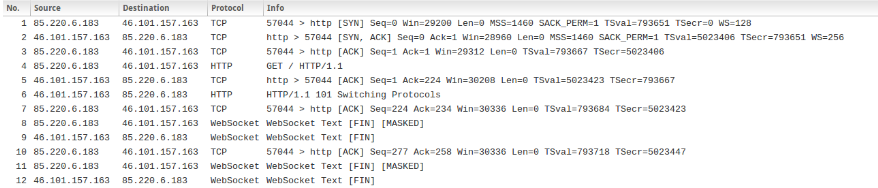
\includegraphics[width=1.2\textwidth]{images/ws_dump}}
	\caption{Network traffic for a \texttt{ws://} connection establishment}
	\label{fig:wsTraffic}
\end{figure}

\noindent
The interesting parts of figure~\ref{fig:wsTraffic} are package No. 4, where the client requests a connection upgrade, and package No. 6 where the server inform the client of a protocol switch to upgrade the connection from HTTP to WebSocket. After the connection establishment, data flows between the client and server using the WebSocket protocol. This kind of network traffic would be filtered in many network environments because of its difference from standard HTTP traffic.
\\
\begin{figure}[h!]
	\centering
	\makebox[\textwidth][c]{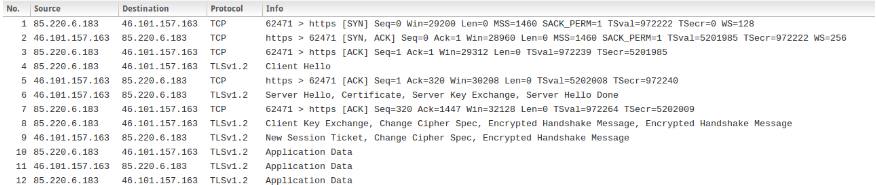
\includegraphics[width=1.2\textwidth]{images/wss_dump}}
	\caption{Network traffic for a \texttt{wss://} connection establishment}
	\label{fig:wssTraffic}
\end{figure}

\noindent
Connection establishment using \texttt{wss://} is largely hidden from network tools like can be seen in figure~\ref{fig:wssTraffic}. This is the reason WebSocket traffic over TLS is more likely to succeed than unencrypted WebSocket traffic. Package No. 4 shows the beginning of the TLS handshake, package No. 6 shows the certificate exchange and package No. 8 shows the key exchange. Afterwards, the application data is encrypted and network intermediaries treat it like regular HTTPS traffic which makes it and other types of encrypted long-lived connections possible.
\\ \\
Figure~\ref{fig:engineioTraffic} shows the process of establishing a bidirectional communication channel with Engine.io which in this case results in a WebSocket connection. The main goals of Engine.io are to provide good performance and user experience across all browsers given the most suitable technologies available at each moment. The reality is that traditional HTTP mechanisms are often capable of providing similarly good user experience like more sophisticated technologies such as WebSocket. The client makes the initial upgrade request to switch to a WebSocket connection in package No. 23. Before making the request the client makes two poll requests in packages No. 4 and 18. Even after the update requests has been made and the server is in the process of of upgrading the request the client makes two more poll requests in packages No. 27 and 43. From package No. 57 and onward a WebSocket connection has been fully established which is at that point considered to be the best mode of communication by Engine.io so it replaces the polling communication. This whole process takes place with out the knowledge of most users and leads to a superior user experience and network utilization than approaches that are fully WebSocket-based or use some form of polling. Based on the experience of the Engine.io developers this procedure is the best approach to establishing an unencrypted WebSocket connection in accordance with the infrastructure of the web.

\begin{figure}[h!]
	\centering
	\makebox[\textwidth][c]{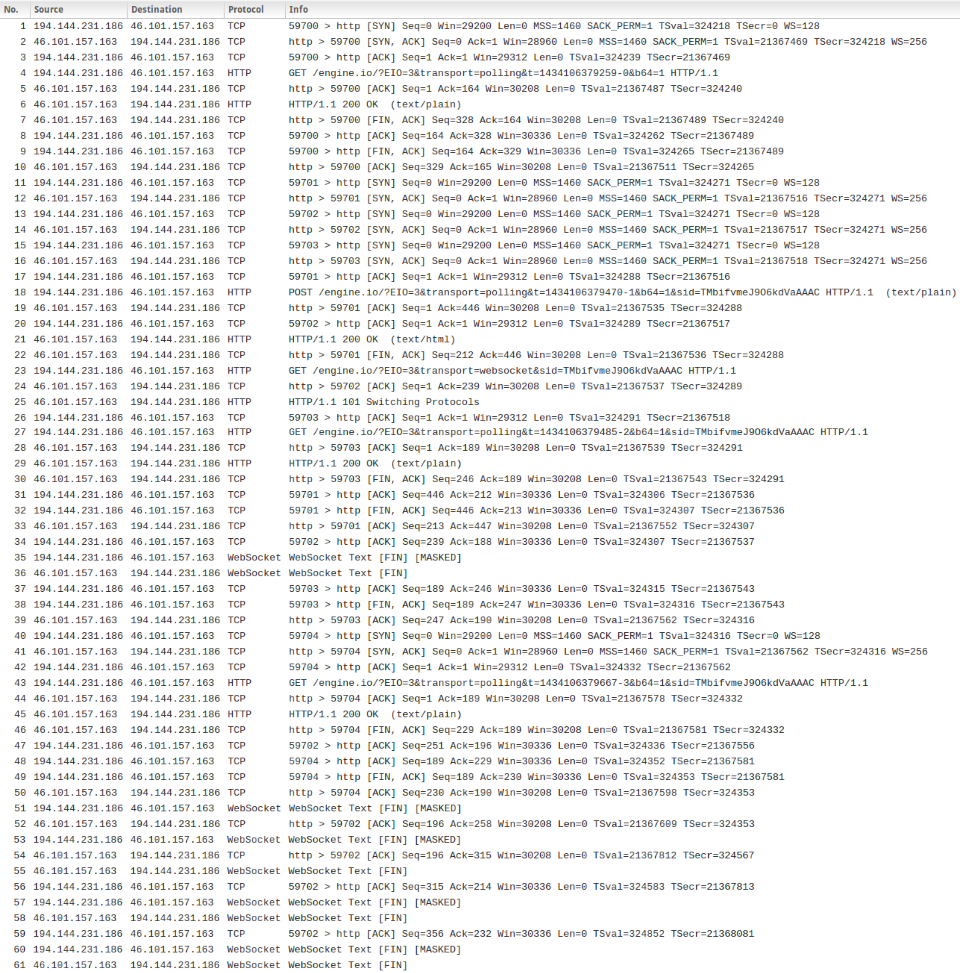
\includegraphics[width=1.2\textwidth]{images/engineio_dump}}
	\caption{Network traffic for an abstracted \texttt{ws://} connection establishment using Engine.io}
	\label{fig:engineioTraffic}
\end{figure}

\section{Containerized WebSocket Infrastructure}

As mentioned in Chapter~\ref{chapter:microservices}, the benefits of deploying applications in containers can be quite appealing compared to more traditional virtualization solutions. Docker\footnote{\url{https://www.docker.com/}} is a platform for the creation and distribution of containers built on top of the existing Linux container technology. In addition to the general benefits of microservices the main advantages of Docker are application portability and the possibility of rapid application deployment. Appendix~\ref{chapter:appendix-binaryTextEchoServer} shows a Dockerfile (instructions used by Docker to automatically build an image) for the text binary echo server used in the WebSocket connection analysis. For the management of more sophisticated "dockerized" infrastructure supporting services such as cluster management, service discovery tools and advanced networking capabilities are needed. Docker and its ecosystem is still relatively young so many of these services are still in early development stages and \textit{de facto} standards are yet to be decided. The recommended best practices and supporting services will most likely go through an adaption phase in the near future as this technology gets more established.


\subsection{Deploying Containerized Infrastructure}

The currently most common way of deploying containers is to use a VM as a host for one or more containers. This method was used to deploy the applications and services developed as a part of this thesis using Ubuntu 14.04.2 LTS as the host system. It is not the ideal solution as it introduces additional overhead and makes scaling more cumbersome later in the deployment process. At the moment this approach seems to be the best one available as it provides more isolation from other users if a shared hosting services is being used for deployment and also makes it possible to reserve kernel resources. Most of the specialized Docker hosting services, offered by the likes of Amazon Web Services and Google, use a similar approach by provisioning a VM that is then used to host the containers even though it is possible to install Docker hosts directly on the underlying hardware which should lead to a better utilization of system resources \cite{mouat2015docker}.
\\ \\
The Docker host must be a Linux OS with kernel version 3.10 or newer which makes distributions like Ubuntu 14.04 LTS \footnote{\url{http://releases.ubuntu.com/14.04/}}, Debian 8\footnote{\url{https://www.debian.org/}} and CentOS 7\footnote{\url{http://www.centos.org/}} into possible candidates as Docker hosts \cite{dockerBinaries}. For larger clusters it might be sensible to use distribution specially intended for hosting containers like CoreOS\footnote{\url{https://coreos.com/}} which provides the minimal functionality required for containerized application deployment. For a cluster of hosts it is practical to use a configuration management tool to management the Docker hosts and images and ensuring that they are up-to-date. The two most common approaches to container management are to treat the containers like VMs whose content can be updated or to view the containers as black boxes that can be replaced but not modified. The advantage of the later approach is that it is easier to keep track of the content of each container through commit tags or a specialized tagging system. Monitoring is another important aspect of container management because the number of run-time environments is usually much greater in systems that are built based on the ideology of microservices. Like with other supporting services in the Docker ecosystem there are multiple available solutions for monitoring suitable for different use cases and best practices are still in the process of being defined.

\subsection{WebSocket-related Deployment Considerations}

In addition to deciding a suitable communication strategy there are other factors that must be taken into consideration when deploying WebSocket applications. Network intermediaries that can impact deployed services are either located on the path between its users and the internet or between its servers and the internet. Most often it is impossible to influence the configuration of the users network and proxies on external networks so communication strategies like the ones that have been mentioned before must be utilized. As the adoption of HTTP/2 increases networks will more commonly be configured to allow long-lived connection which will increase the effectiveness of the WebSocket protocol. Infrastructure on the serving path that can be configured and is intended for WebSocket traffic should be tuned for long-lived connections. That is something that takes special care as most network infrastructure is configured by default for short lived HTTP traffic. Nginx for example is configured to timeout connections that have been idle for 60 seconds unless the timeout interval is specially increase like can be seen in the configuration file in Appendix~\ref{chapter:chapter:appendix-reverseProxy}. The number of expected concurrent connections must also be taken into account as most Unix systems have a pre-configured limit on the number of open sockets. This limit can be seen with the \texttt{ulimit -a} command and is usually set at 1024. To increase the limit the \texttt{-n} flag can be used (\texttt{ulimit -n 2048} to double the default limit of allowed concurrent sockets). Other areas of consideration include identifying critical areas more monitoring, introducing ping intervals to prevent connection timeouts and identifying where throttling might improve performance. WebSocket-based applications introduce a range of operational challenges not associated with HTTP-based applications that must be dealt with accordingly if the benefits of the protocol are to be fully reaped.